
%%%%%%%%%%%%%%%%
%%%%%%%%%%%%%%%%

\section{Simple DEC analysis} \label{sec:bg_simple}


The following series of tutorials will estimate the ancestral ranges of the silversword alliance (Tribe {\it Madiinae}), a young and diverse clade of about 50 species and subspecies.
Although silverswords are endemic to Hawaii, they are nested within a larger clade alongside tarweeds, which are native to western continental North America \citep{Baldwin1991}.
The size and age of the silversword clade, combined with our knowledge of Hawaiian island formation, makes it an ideal system to explore concepts in historical biogeography and phylogeny.
For further reading, consult: \citet{Carlquist1959, Baldwin1998}.
 
\begin{figure}[!ht]
\centering
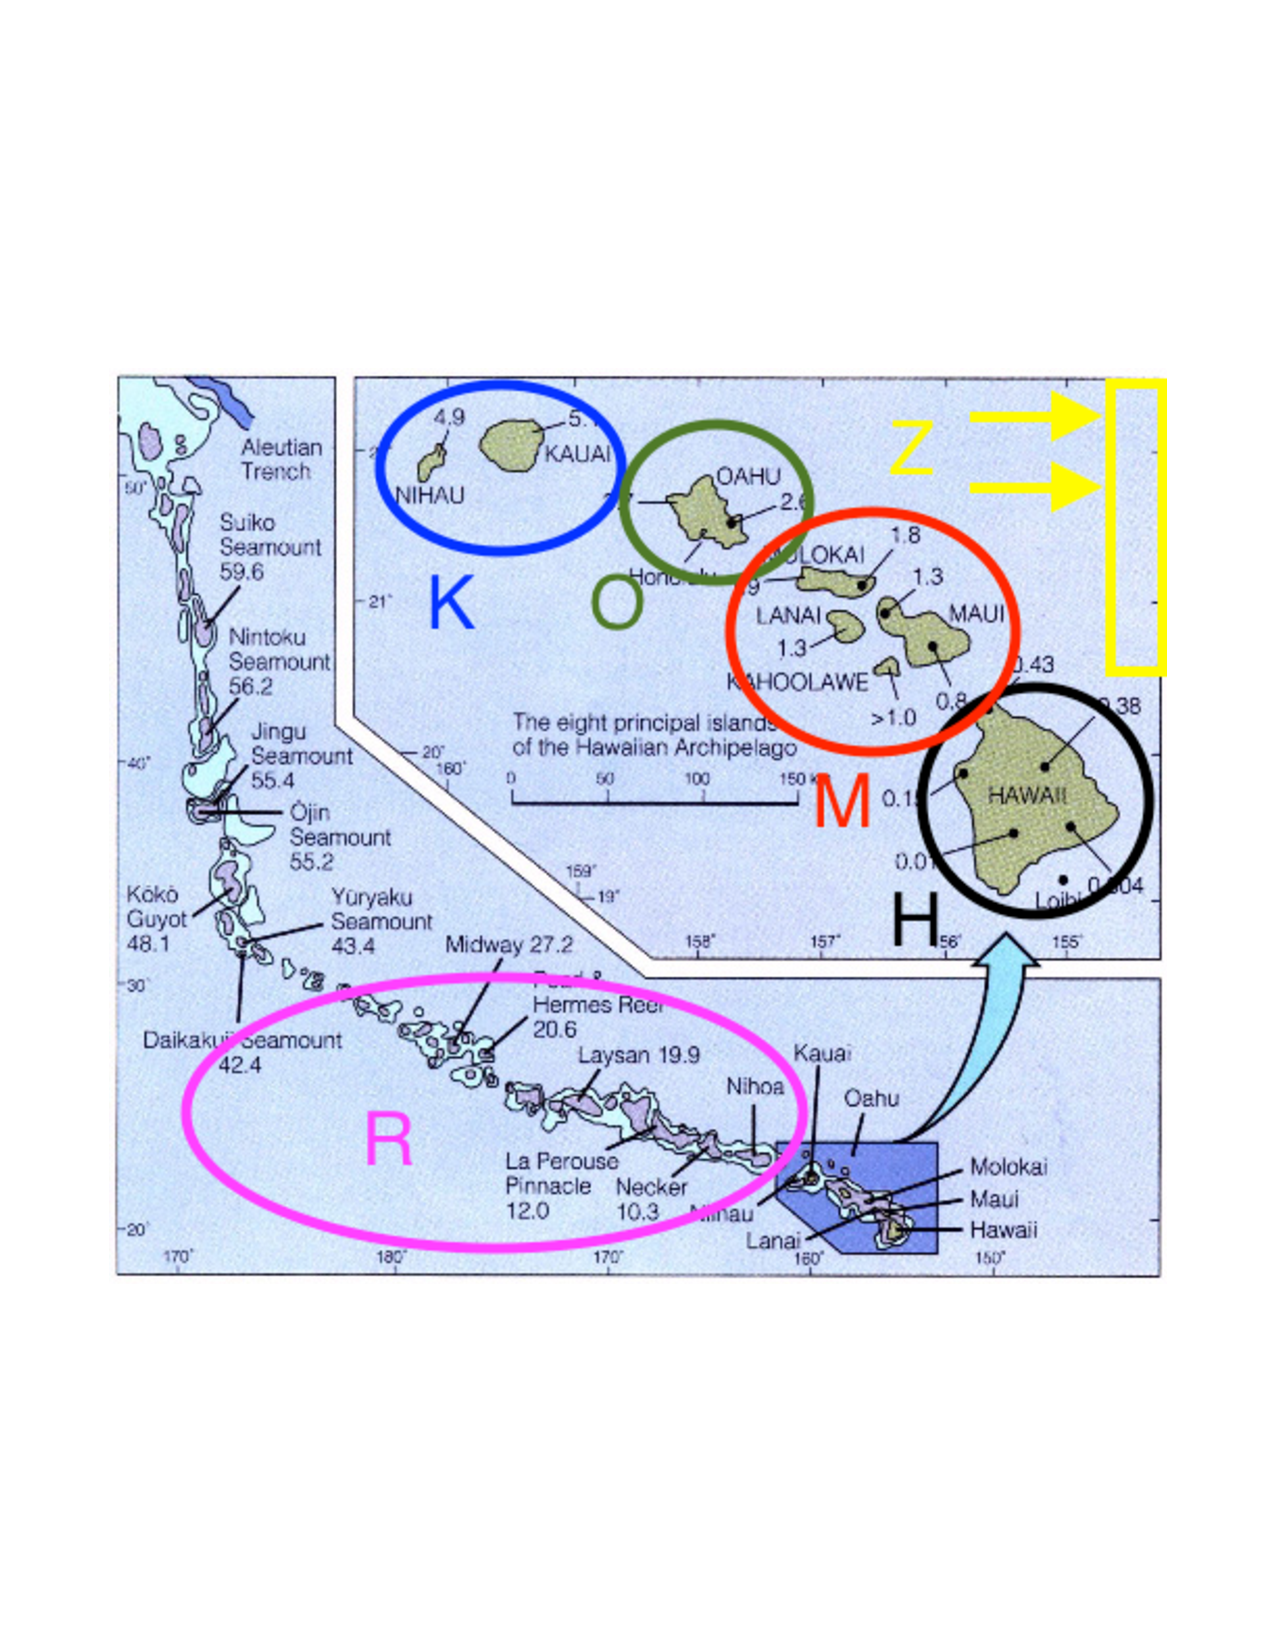
\includegraphics[width=0.6\textwidth]{figures/fig_hawaii_areas.pdf}
\caption{A beautiful figure of the discrete areas for the tutorial. Six areas are shown: Kauai and Niihau (K); Oahu (O); Maui-Nui, Lanai, and Molokai (M); Hawaii (H); the remaining Hawaiian islands (R); and the North American mainland (Z).}
\label{fig:hawaii_areas}
\end{figure}
 
For this tutorial we'll focus entirely on the silversword alliance and the modern Hawaiian archipelago.
To begin, we'll use just four areas, K, O, M, and H, and include areas R and Z in later analyses (Figure \ref{fig:hawaii_areas}).
The species ranges used in this exercise follow \citet{Gillespie2009}.

\begin{table}[!ht]
\centering
\scriptsize
\begin{tabular}{llcc}
Range & Areas & Size & State \\ \hline
$\emptyset$ & 0000 & 0 & 0 \\
K    & 1000 & 1 & 1 \\
O    & 0100 & 1 & 2 \\
M    & 0010 & 1 & 3 \\
H    & 0001 & 1 & 4 \\
KO   & 1100 & 2 & 5 \\
KM   & 1010 & 2 & 6 \\
OM   & 0110 & 2 & 7 \\
KH   & 1001 & 2 & 8 \\
OH   & 0101 & 2 & 9 \\
MH   & 0011 & 2 & 10 \\
KOM  & 1110 & 3 & 11 \\ 
KOH  & 1101 & 3 & 12 \\
KMH  & 1011 & 3 & 13 \\
OMH  & 0111 & 3 & 14 \\
KOMH & 1111 & 4 & 15 \\
\end{tabular}
\caption{Area coding used for four areas: K is Kauai and Nihoa; O is Oahu; M is Maui Nui, Lanai, and Molokai; H is Hawaii island.}
\end{table}

\subsection*{Analysis}

First, create file management variables for input and output

\begin{snugshade*}
\begin{lstlisting}
range_fn = "data/n4/silversword.n4.range.nex"
tree_fn = "data/n4/silversword.tre"
out_fn = "output/simple"
\end{lstlisting}
\end{snugshade*}

then read in our character data as binary presence-absence characters

\begin{snugshade}
\begin{lstlisting}
dat_range_01 = readDiscreteCharacterData(range_fn)
\end{lstlisting}
\end{snugshade}

then encode the species ranges into natural numbers

\begin{snugshade}
\begin{lstlisting}
dat_range_n    = formatDiscreteCharacterData(dat_range_01, "DEC")
\end{lstlisting}
\end{snugshade}


Record the number of areas (characters) from the discrete character data object

\begin{snugshade}
\begin{lstlisting}
n_areas = dat_range_01.nchar()
\end{lstlisting}
\end{snugshade}

You can view the taxon data to see how characters are coded both as human-readable presence-absence data and as computer-readable natural numbers
\begin{snugshade}
\begin{lstlisting}
dat_range_01[1]
|*  Argyroxiphium_grayanum_East_Maui:
|*    0010
dat_range_n[1]
|*  Argyroxiphium_grayanum_East_Maui:
|*    3
\end{lstlisting}
\end{snugshade}

For this tutorial we'll assume we know the dated species phylogeny without error.

\begin{snugshade}
\begin{lstlisting}
tree <- readTrees(tree_fn)[1]
\end{lstlisting}
\end{snugshade}

Next, we'll build the anagenetic rate matrix for the DEC model.
In its simplest form, the rate matrix requires a dispersal rate and an extirpation rate.
For this analysis, we'll assume that all pairs of areas share the same dispersal rate and all areas share the same extirpation rate.
To gain greater control to observe and manage prior sensitivity, we'll reparameterize the DEC rate matrix to report the {\it relative} rates of dispersal versus extirpation events.
In order for anagenetic event rates to be measured on an absolute time scale (e.g. in millions of years), we will also introduce a a biogeographic rate parameter, similar to the molecular clock parameter used in dating analyses.

First, create a parameter for the arrival rate of anagenetic range evolution events.
We'll apply an uninformative prior to the rate's magnitude by first assigning a uniform distribution to the log$_{10}$ rate.

\begin{snugshade}
\begin{lstlisting}
log10_rate_bg ~ dnUniform(-4,2)
log10_rate_bg.setValue(-2)
moves[1] = mvSlide(log10_rate_bg, weight=4)
\end{lstlisting}
\end{snugshade}

then convert the rate from log-scale to linear-scale with a deterministic node

\begin{snugshade}
\begin{lstlisting}
rate_bg := 10^log10_rate_bg
\end{lstlisting}
\end{snugshade}

This yields a uniform prior over orders of magnitude, ranging from $10^{-4}$ to $10^2$ events per million years.

Because the rate matrix will describe the relative anagenetic event rates, we can safely assume that dispersal occurs at the relative (fixed) rate of one.

\begin{snugshade}
\begin{lstlisting}
dispersal_rate <- abs(1)
\end{lstlisting}
\end{snugshade}

then create the dispersal rate matrix

\begin{snugshade}
\begin{lstlisting}
for (i in 1:n_areas) {
  for (j in 1:n_areas) {
    dr[i][j] <- dispersal_rate
  }
}
\end{lstlisting}
\end{snugshade}

Next, assign a prior distribution to the relative extirpation rate and assign it a move.
The prior distribution of extirpation rates is given {\tt log\_sd} and {\tt log\_mean} values that give the prior expected value of one -- i.e. the mean rate of area gain and area loss are equal under the prior.

\begin{snugshade}
\begin{lstlisting}
log_sd <- 0.5
log_mean <- ln(1) - 0.5*log_sd^2
extirpation_rate ~ dnLognormal(mean=log_mean, sd=log_sd)
moves[2] = mvScale(extirpation_rate, weight=2)
\end{lstlisting}
\end{snugshade}

then create a matrix of extirpation rates

\begin{snugshade}
\begin{lstlisting}
for (i in 1:n_areas) {
  for (j in 1:n_areas) {
    er[i][j] <- abs(0)        
  }
  er[i][i] := extirpation_rate
}
\end{lstlisting}
\end{snugshade}

Note that {\tt er} is a diagonal matrix whose diagonal values are determined ({\tt :=}) by the stochastic variable, {\tt extirpation\_rate}.
We can now create our relative rate matrix, {\tt Q\_DEC}, with the {\tt fnDECRateMatrix} function.

\begin{snugshade}
\begin{lstlisting}
Q_DEC := fnDECRateMatrix(dispersalRates=dr, extirpationRates=er)
\end{lstlisting}
\end{snugshade}

Note, {\tt fnDECRateMatrix} does not rescale its elements in any way, so transition rates share the same time scale as the underlying tree.
%In our case, the tree is measured in millions of years (Ma).
This scaling is in contrast to the standard molecular substitution processes that are available in \RevBayes, such as {\tt fnGTR}, whose rates are rescaled such that the process is expected to produce one event per site per unit time.

Next, we need to create the cladogenetic probability matrix.
Cladogenetic event probabilities are given by a transition probability matrix, not a rate matrix.
First, we will provide the vector {\tt [ ``s'', ``a'' ]} to indicate that we wish to consider only subset sympatry and allopatry events.
Next, we will create a vector of prior weights on cladogenesis events that fixes all cladogenetic events to be equiprobable.

\begin{snugshade}
\begin{lstlisting}
clado_event_types <- [ "s", "a" ]
clado_event_probs <- simplex(1, 1)
P_DEC := fnDECCladoProbs(eventProbs=clado_event_probs,
                            eventTypes=clado_event_types,
                            numCharacters=n_areas)
\end{lstlisting}
\end{snugshade}

Finally, all our DEC model components are encapsulated in the {\tt dnPhyloCTMCClado} distribution, which is similar to {\tt dnPhyloCTMC} except specialized to integrate over cladogenetic events.
Although this dataset has four areas, it is recognized single character with states valued from 1 to $2^4$, hence {\tt nSites=1}.

\begin{snugshade}
\begin{lstlisting}
m_bg ~ dnPhyloCTMCClado(tree=tree,
                           Q=Q_DEC,
                           cladoProbs=P_DEC,
                           branchRates=rate_bg,
                           nSites=1,
                           type="NaturalNumbers")
\end{lstlisting}
\end{snugshade}

Finally, attach the observed ranges to the model.
Be sure to use the natural number valued range characters, {\tt dat\_range\_n}, and not the presence-absence range characters, {\tt dat\_range\_01}.

\begin{snugshade}
\begin{lstlisting}
m_bg.clamp(dat_range_n)
\end{lstlisting}
\end{snugshade}

Add the monitors.

\begin{snugshade}
\begin{lstlisting}
monitors[1] = mnScreen(rate_bg, extirpation_rate, printgen=100)
monitors[2] = mnModel(file=out_fn+".params.log", printgen=10)
monitors[3] = mnFile(tree, file=out_fn+".tre", printgen=10)
monitors[4] = mnJointConditionalAncestralState(tree=tree,
                                                    ctmc=m_bg,
                                                    filename=out_fn+".states.log",
                                                    type="NaturalNumbers",
                                                    printgen=10,
                                                    withTips=true,
                                                    withStartStates=true)
\end{lstlisting}
\end{snugshade}

The {\tt mnJointConditionalAncestralState} monitor samples ancestral states from the phylogeny, {\tt tree}, according to the model of evolution, {\tt m\_bg}, and stores it to the file named {\tt "simple.states.log"}.
Each row in the states file lists the joint sample of ancestral states conditioned on the tip values for the entire tree (i.e. a {\it joint} ancestral state sample {\it conditional} on the tip states).
Each column corresponds to the phylogenetic node index for that particular MCMC sample.
The index is used used to match the state samples with the tree samples, which is especially important when the topology is a random variable (Section \ref{sec:bg_phylo}).

The remaining tasks should be familiar from previous tutorials, so we can proceed briskly.
Prepare the model graph for analysis by creating a {\tt Model} object.
\begin{snugshade}
\begin{lstlisting}
mymodel = model(m_bg)
\end{lstlisting}
\end{snugshade}


Create the {\tt MCMC} object from the model, moves, and monitors variables, and run the MCMC analysis.
\begin{snugshade}
\begin{lstlisting}
mymcmc = mcmc(mymodel, moves, monitors)
mymcmc.run(3000)
\end{lstlisting}
\end{snugshade}

\subsection*{Results}

\begin{center}
{\it Example results are located at \tt{output\_example/simple.*}}
\end{center}

The script located at {\tt scripts/make\_anc\_states.Rev} contains code to construct an ancestral state tree.
Like all \RevBayes scripts, this script may be executed from the command line.
Because this is the first time using the script, we'll enter the code manually.
To use it for future analyses, just modify the {\tt out\_str} variable to match the prefix of the target analysis, save the file, then execute the script by typing {\tt "rb scripts/make\_anc\_states.Rev"} into the command line.

\begin{figure}[!h]
\centering
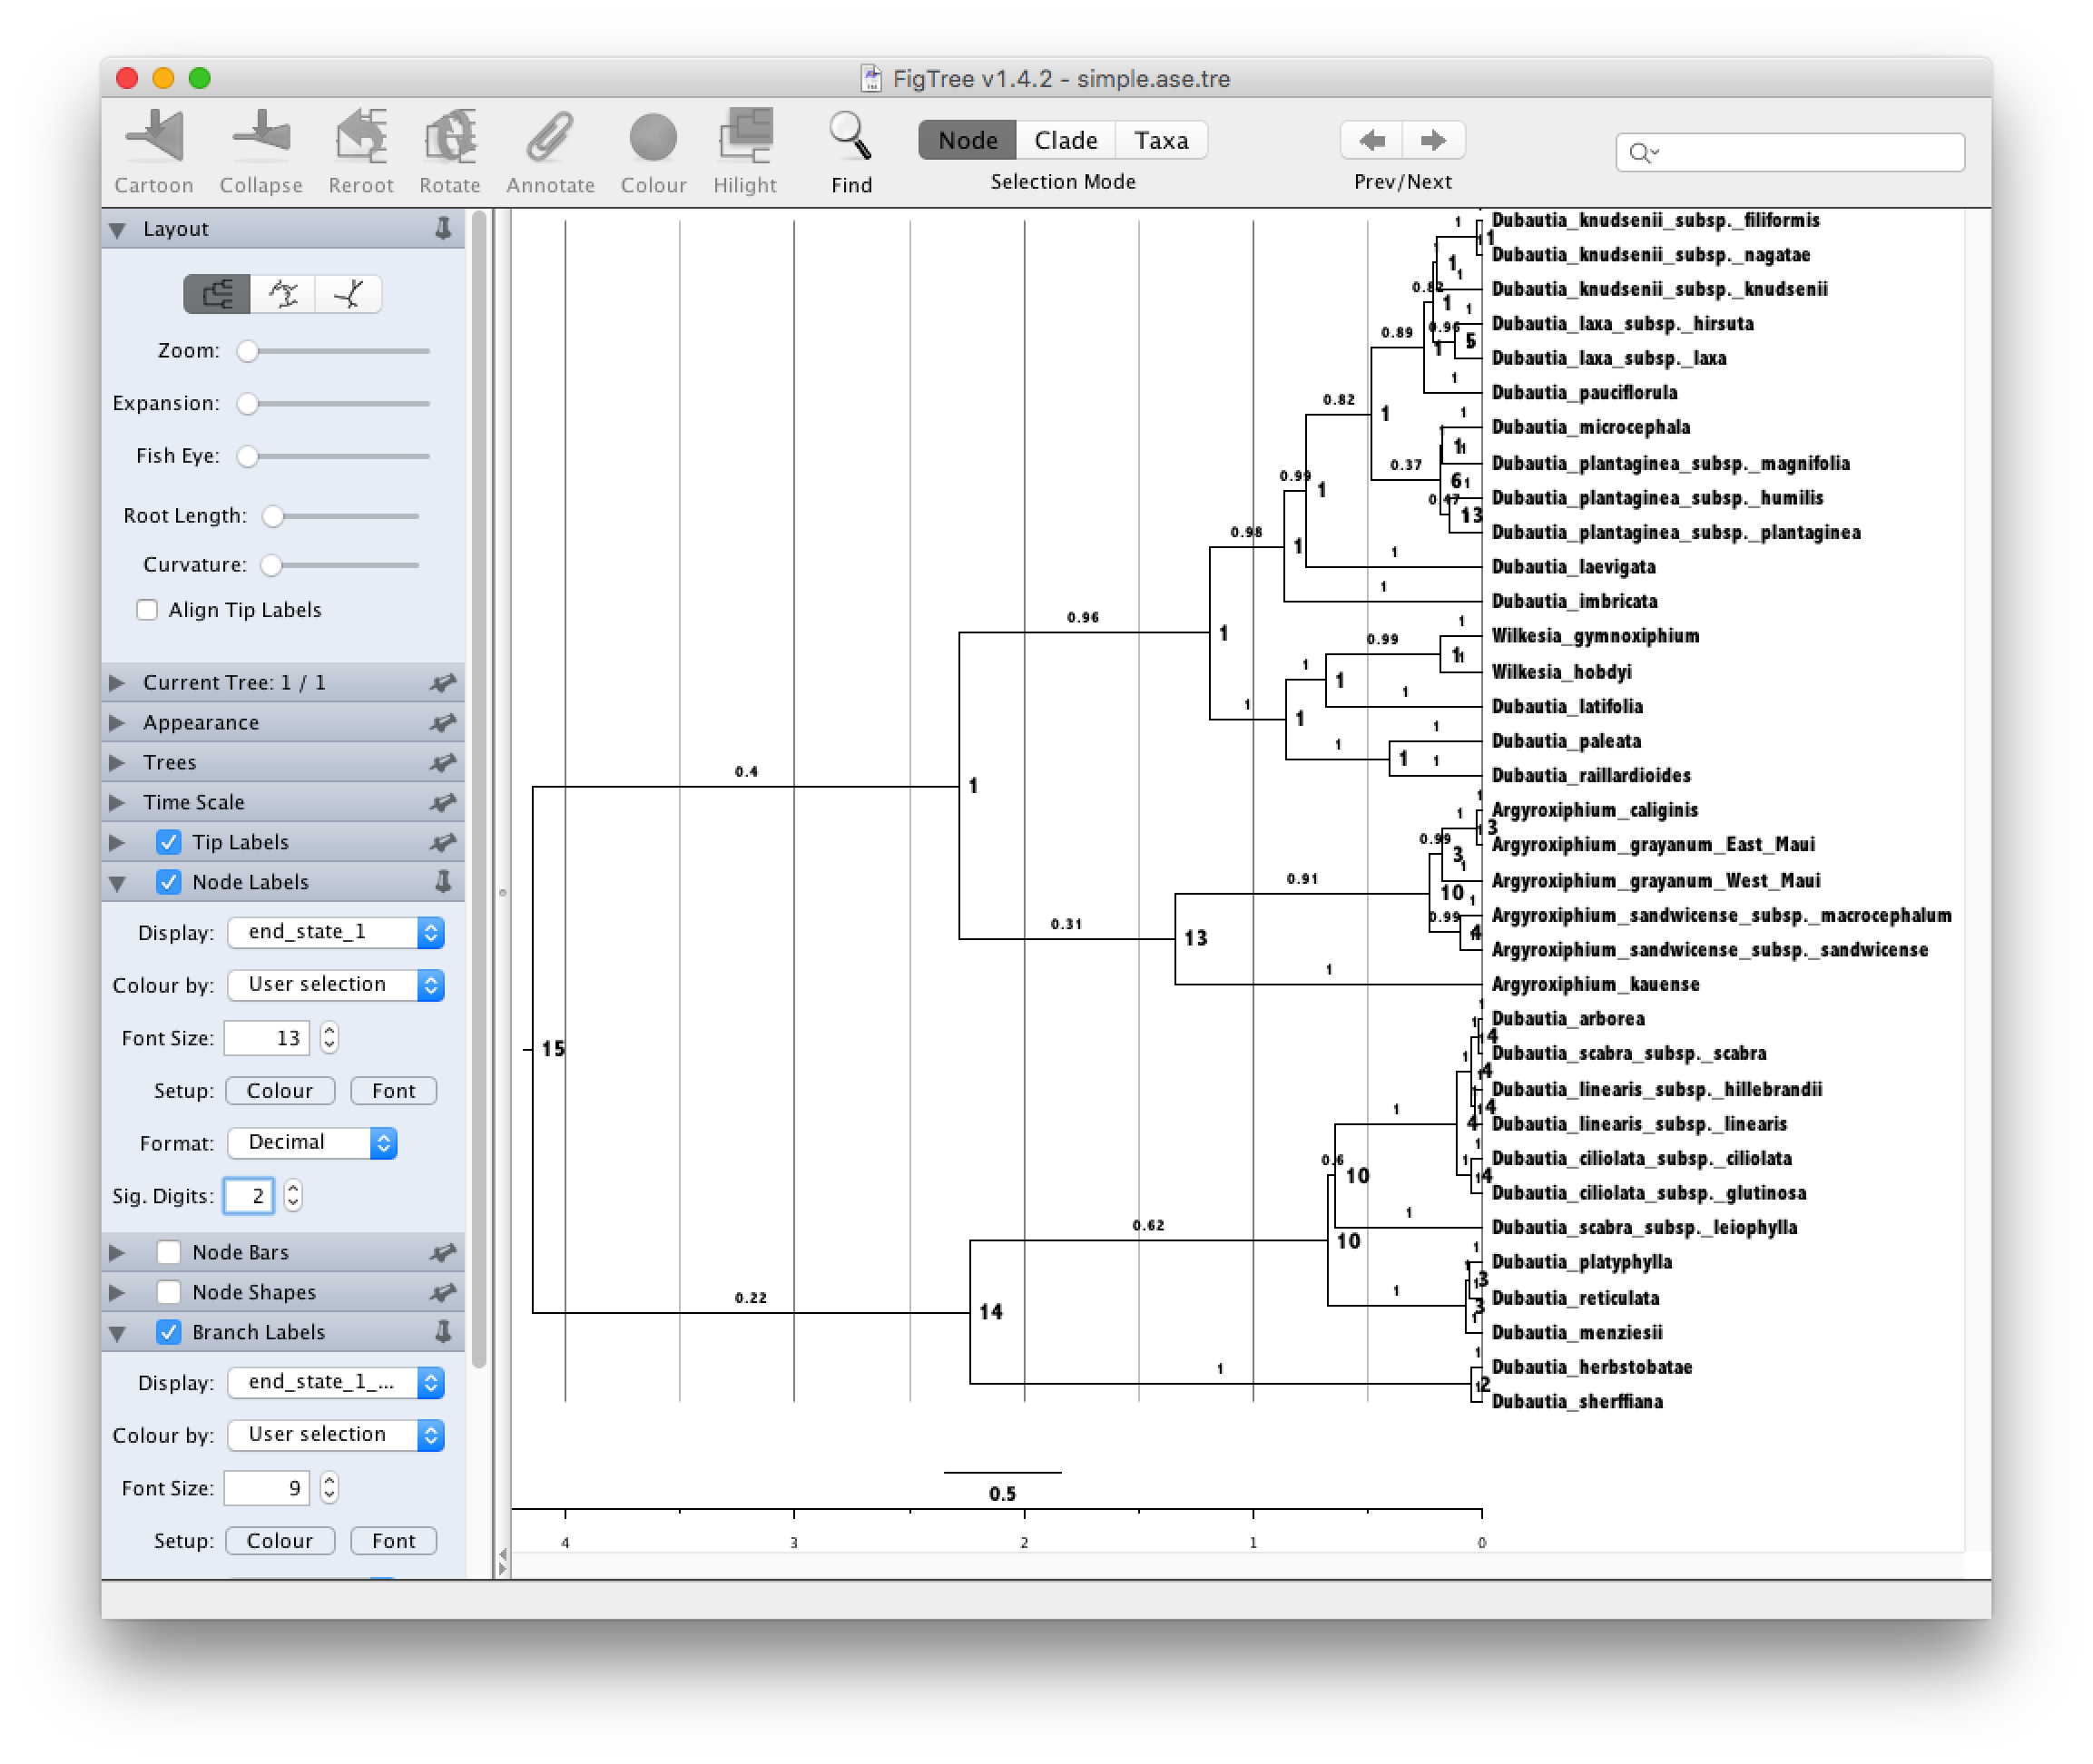
\includegraphics[width=0.9\textwidth]{figures/fig_simple_FigTree_ase.png}
\caption{Annotated tree with ancestral state estimates in \FigTree.
This tree was generated by {\tt ancestralStateTree} in \RevBayes.
The most probable end state of each branch (before cladogenesis) is shown at each node.
Branches are labeled with the posterior probability for the ancestral state on the tipwards end of the branch.
}
\label{fig:simple_FigTree_ase}
\end{figure}

After opening a new \RevBayes session, create helper variables for files we'll work with.
\begin{snugshade}
\begin{lstlisting}
out_str = "output/simple"
out_state_fn = out_str + ".states.log"
out_tree_fn = out_str + ".tre"
out_mcc_fn = out_str + ".mcc.tre" 
\end{lstlisting}
\end{snugshade}

Build a maximum clade credibility tree from the posterior tree distribution, discarding the first 25\% of samples.
(Note, this step is gratuitous when we assume a fixed phylogeny, but essential when we estimate the phylogeny in Section \ref{sec:bg_phylo}).

\begin{snugshade}
\begin{lstlisting}
tree_trace = readTreeTrace(file=out_tree_fn, treetype="clock")
tree_trace.setBurnin(0.25)
n_burn = tree_trace.getBurnin()
\end{lstlisting}
\end{snugshade}

Compute and save the maximum clade credibility tree
\begin{snugshade}
\begin{lstlisting}
mcc_tree = mccTree(tree_trace, file=out_mcc_fn)
\end{lstlisting}
\end{snugshade}

Get the ancestral state trace from {\tt simple.states.log}

\begin{snugshade}
\begin{lstlisting}
state_trace = readAncestralStateTrace(file=out_state_fn)
\end{lstlisting}
\end{snugshade}


Get the ancestral state tree trace from {\tt simple.tre}.
It is important to use {\tt readAncestralTreeTrace} and not {\tt readTreeTrace} to properly annotate the tree with ancestral states.

\begin{snugshade}
\begin{lstlisting}
tree_trace = readAncestralStateTreeTrace(file=out_tree_fn, treetype="clock")
\end{lstlisting}
\end{snugshade}

Finally, compute and save the ancestral state tree as {\tt simple.ase.tre}.

\begin{snugshade}
\begin{lstlisting}
anc_tree = ancestralStateTree(tree=mcc_tree,
                              ancestral_state_trace_vector=state_trace,
                              tree_trace=tree_trace,
                              include_start_states=true,
                              file=out_str+".ase.tre",
                              burnin=n_burn,
                              site=0)
\end{lstlisting}
\end{snugshade}

We can review the output from {\tt ancestralStateTree} in \FigTree (Figure \ref{fig:simple_FigTree_ase}).

Ancestral state trees are annotated with the first three most probable ancestral states along with their posterior probabilities.
When the tree is a random variable, as it is in later exercises, additional information about phylogenetic uncertainty is reported.

Finally, we can also generate a figure with ancestral states that is suitable for publication using the \R package {\tt RevGadgets} (Figure \ref{fig:simple_RevGadgets_ase}).
The script is easily modified for use with different datasets.
To create build a figure, open an \R session and load the plotting script with the {\tt source} function
\begin{snugshade}
\begin{lstlisting}
source("plot_anc_state.n4.R")
\end{lstlisting}
\end{snugshade}

\begin{figure}[!h]
\centering
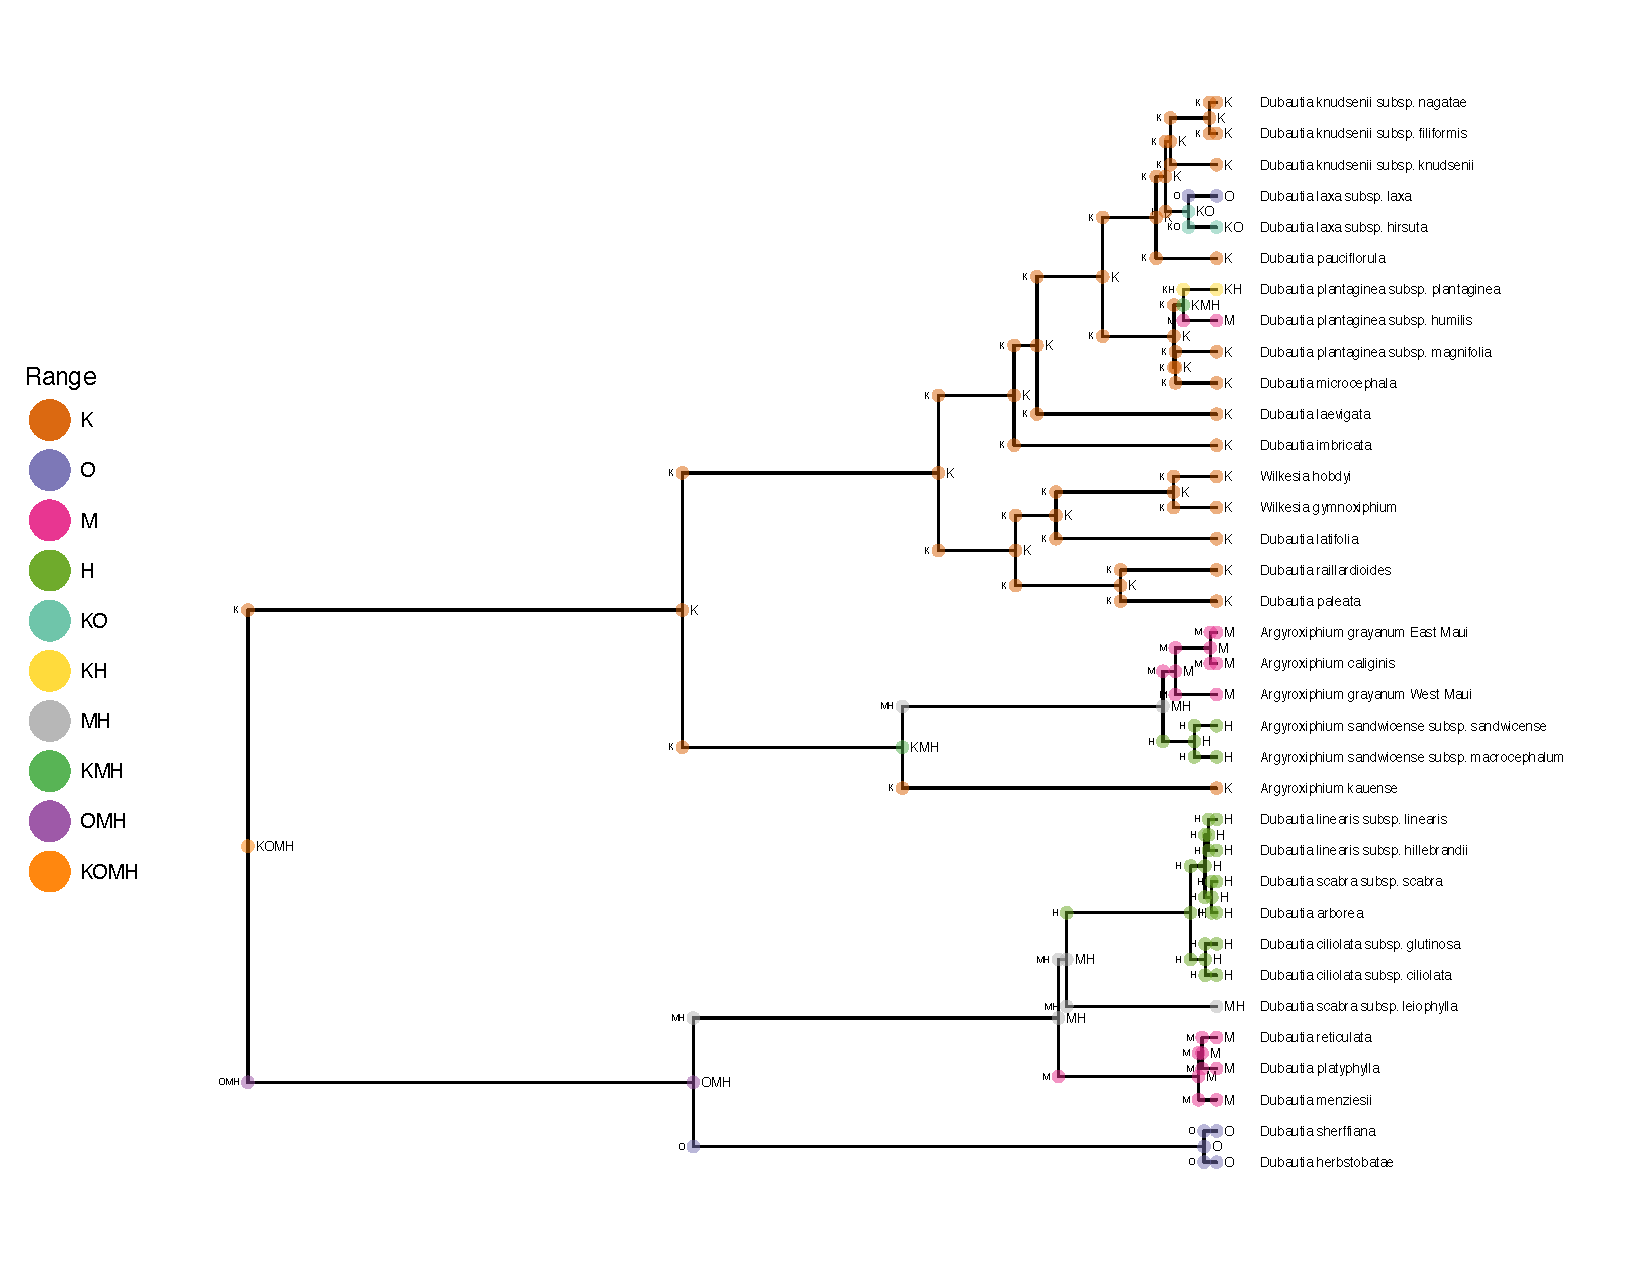
\includegraphics[width=0.75\textwidth]{figures/fig_simple_RevGadgets_ase.pdf}
\caption{Tree with ancestral state estimates for the ``simple'' analysis. Nodes are annotated with ancestral states before and after cladogenetic events. The ancestral range with the highest posterior probability is shown. Colors of markers indicate the range state.}
\label{fig:simple_RevGadgets_ase}
\end{figure}

Notice that the model infers a widespread ancestral range for the clade (KOMH) approximately four million years ago when only Kauai existed.
Similar geologically unrealistic widespread ranges are estimated for the {\it Agyroxiphium} clade (KMH) and the {\it D. sheriffiana} and {\it D. arborea} clade (OMH).
The remaining tutorials will focus on improvements to the simple DEC model presented here.

\newpage
